% Options for packages loaded elsewhere
\PassOptionsToPackage{unicode}{hyperref}
\PassOptionsToPackage{hyphens}{url}
%


\PassOptionsToPackage{table}{xcolor}

\documentclass[
  10pt,
  letterpaper,
]{article}

\usepackage{amsmath,amssymb}
\usepackage{lmodern}
\usepackage{iftex}
\ifPDFTeX
  \usepackage[T1]{fontenc}
  \usepackage[utf8]{inputenc}
  \usepackage{textcomp} % provide euro and other symbols
\else % if luatex or xetex
  \usepackage{unicode-math}
  \defaultfontfeatures{Scale=MatchLowercase}
  \defaultfontfeatures[\rmfamily]{Ligatures=TeX,Scale=1}
\fi
% Use upquote if available, for straight quotes in verbatim environments
\IfFileExists{upquote.sty}{\usepackage{upquote}}{}
\IfFileExists{microtype.sty}{% use microtype if available
  \usepackage[]{microtype}
  \UseMicrotypeSet[protrusion]{basicmath} % disable protrusion for tt fonts
}{}
\makeatletter
\@ifundefined{KOMAClassName}{% if non-KOMA class
  \IfFileExists{parskip.sty}{%
    \usepackage{parskip}
  }{% else
    \setlength{\parindent}{0pt}
    \setlength{\parskip}{6pt plus 2pt minus 1pt}}
}{% if KOMA class
  \KOMAoptions{parskip=half}}
\makeatother
\usepackage{xcolor}
\usepackage[top=0.85in,left=2.75in,footskip=0.75in]{geometry}
\setlength{\emergencystretch}{3em} % prevent overfull lines
\setcounter{secnumdepth}{-\maxdimen} % remove section numbering


\providecommand{\tightlist}{%
  \setlength{\itemsep}{0pt}\setlength{\parskip}{0pt}}\usepackage{longtable,booktabs,array}
\usepackage{calc} % for calculating minipage widths
% Correct order of tables after \paragraph or \subparagraph
\usepackage{etoolbox}
\makeatletter
\patchcmd\longtable{\par}{\if@noskipsec\mbox{}\fi\par}{}{}
\makeatother
% Allow footnotes in longtable head/foot
\IfFileExists{footnotehyper.sty}{\usepackage{footnotehyper}}{\usepackage{footnote}}
\makesavenoteenv{longtable}
\usepackage{graphicx}
\makeatletter
\def\maxwidth{\ifdim\Gin@nat@width>\linewidth\linewidth\else\Gin@nat@width\fi}
\def\maxheight{\ifdim\Gin@nat@height>\textheight\textheight\else\Gin@nat@height\fi}
\makeatother
% Scale images if necessary, so that they will not overflow the page
% margins by default, and it is still possible to overwrite the defaults
% using explicit options in \includegraphics[width, height, ...]{}
\setkeys{Gin}{width=\maxwidth,height=\maxheight,keepaspectratio}
% Set default figure placement to htbp
\makeatletter
\def\fps@figure{htbp}
\makeatother

% Use adjustwidth environment to exceed column width (see example table in text)
\usepackage{changepage}

% marvosym package for additional characters
\usepackage{marvosym}

% cite package, to clean up citations in the main text. Do not remove.
% Using natbib instead
% \usepackage{cite}

% Use nameref to cite supporting information files (see Supporting Information section for more info)
\usepackage{nameref,hyperref}

% line numbers
\usepackage[right]{lineno}

% ligatures disabled
\usepackage{microtype}
\DisableLigatures[f]{encoding = *, family = * }

% create "+" rule type for thick vertical lines
\newcolumntype{+}{!{\vrule width 2pt}}

% create \thickcline for thick horizontal lines of variable length
\newlength\savedwidth
\newcommand\thickcline[1]{%
  \noalign{\global\savedwidth\arrayrulewidth\global\arrayrulewidth 2pt}%
  \cline{#1}%
  \noalign{\vskip\arrayrulewidth}%
  \noalign{\global\arrayrulewidth\savedwidth}%
}

% \thickhline command for thick horizontal lines that span the table
\newcommand\thickhline{\noalign{\global\savedwidth\arrayrulewidth\global\arrayrulewidth 2pt}%
\hline
\noalign{\global\arrayrulewidth\savedwidth}}

% Text layout
\raggedright
\setlength{\parindent}{0.5cm}
\textwidth 5.25in 
\textheight 8.75in

% Bold the 'Figure #' in the caption and separate it from the title/caption with a period
% Captions will be left justified
\usepackage[aboveskip=1pt,labelfont=bf,labelsep=period,justification=raggedright,singlelinecheck=off]{caption}
\renewcommand{\figurename}{Fig}

% Remove brackets from numbering in List of References
\makeatletter
\renewcommand{\@biblabel}[1]{\quad#1.}
\makeatother

% Header and Footer with logo
\usepackage{lastpage,fancyhdr}
\usepackage{epstopdf}
%\pagestyle{myheadings}
\pagestyle{fancy}
\fancyhf{}
%\setlength{\headheight}{27.023pt}
%\lhead{\includegraphics[width=2.0in]{PLOS-submission.eps}}
\rfoot{\thepage/\pageref{LastPage}}
\renewcommand{\headrulewidth}{0pt}
\renewcommand{\footrule}{\hrule height 2pt \vspace{2mm}}
\fancyheadoffset[L]{2.25in}
\fancyfootoffset[L]{2.25in}
\lfoot{\today}
\makeatletter
\makeatother
\makeatletter
\makeatother
\makeatletter
\@ifpackageloaded{caption}{}{\usepackage{caption}}
\AtBeginDocument{%
\ifdefined\contentsname
  \renewcommand*\contentsname{Table of contents}
\else
  \newcommand\contentsname{Table of contents}
\fi
\ifdefined\listfigurename
  \renewcommand*\listfigurename{List of Figures}
\else
  \newcommand\listfigurename{List of Figures}
\fi
\ifdefined\listtablename
  \renewcommand*\listtablename{List of Tables}
\else
  \newcommand\listtablename{List of Tables}
\fi
\ifdefined\figurename
  \renewcommand*\figurename{Figure}
\else
  \newcommand\figurename{Figure}
\fi
\ifdefined\tablename
  \renewcommand*\tablename{Table}
\else
  \newcommand\tablename{Table}
\fi
}
\@ifpackageloaded{float}{}{\usepackage{float}}
\floatstyle{ruled}
\@ifundefined{c@chapter}{\newfloat{codelisting}{h}{lop}}{\newfloat{codelisting}{h}{lop}[chapter]}
\floatname{codelisting}{Listing}
\newcommand*\listoflistings{\listof{codelisting}{List of Listings}}
\makeatother
\makeatletter
\@ifpackageloaded{caption}{}{\usepackage{caption}}
\@ifpackageloaded{subcaption}{}{\usepackage{subcaption}}
\makeatother
\makeatletter
\makeatother
\ifLuaTeX
  \usepackage{selnolig}  % disable illegal ligatures
\fi
\usepackage[numbers,square,comma]{natbib}
\bibliographystyle{plos2015}
\IfFileExists{bookmark.sty}{\usepackage{bookmark}}{\usepackage{hyperref}}
\IfFileExists{xurl.sty}{\usepackage{xurl}}{} % add URL line breaks if available
\urlstyle{same} % disable monospaced font for URLs
\hypersetup{
  pdftitle={Working Paper},
  pdfauthor={Witek ten Hove; Ger Koole; Joost Berkhout},
  hidelinks,
  pdfcreator={LaTeX via pandoc}}



\begin{document}
\vspace*{0.2in}

% Title must be 250 characters or less.
\begin{flushleft}
{\Large
\textbf\newline{Working
Paper} % Please use "sentence case" for title and headings (capitalize only the first word in a title (or heading), the first word in a subtitle (or subheading), and any proper nouns).
}
\newline
\\
% Insert author names, affiliations and corresponding author email (do not include titles, positions, or degrees).
Witek ten Hove\textsuperscript{1,2\Yinyang}, Ger
Koole\textsuperscript{2\Yinyang}, Joost
Berkhout\textsuperscript{2\Yinyang}
\\
\bigskip
\textbf{1} Lectoraat Logistiek en Allianties, HAN University of Applied
Sciences, Arnhem, The Netherlands, \\ \textbf{2} Department of
Mathematics, VU, Amsterdam, The Netherlands, 
\bigskip

% Insert additional author notes using the symbols described below. Insert symbol callouts after author names as necessary.
% 
% Remove or comment out the author notes below if they aren't used.
%
% Primary Equal Contribution Note
\Yinyang These authors contributed equally to this work.

% Additional Equal Contribution Note
% Also use this double-dagger symbol for special authorship notes, such as senior authorship.
%\ddag These authors also contributed equally to this work.

% Current address notes
\textcurrency Current Address: Dept/Program/Center, Institution Name, City, State, Country % change symbol to "\textcurrency a" if more than one current address note
% \textcurrency b Insert second current address 
% \textcurrency c Insert third current address

% Deceased author note
\dag Deceased

% Group/Consortium Author Note
\textpilcrow Membership list can be found in the Acknowledgments
sections

% Use the asterisk to denote corresponding authorship and provide email address in note below.

\end{flushleft}

\section*{Abstract}
Lorem ipsum dolor sit amet, consectetur adipiscing elit. Curabitur eget
porta erat. Morbi consectetur est vel gravida pretium. Suspendisse ut
dui eu ante cursus gravida non sed sem. Nullam sapien tellus, commodo id
velit id, eleifend volutpat quam. Phasellus mauris velit, dapibus
finibus elementum vel, pulvinar non tellus. Nunc pellentesque pretium
diam, quis maximus dolor faucibus id. Nunc convallis sodales ante, ut
ullamcorper est egestas vitae. Nam sit amet enim ultrices, ultrices elit
pulvinar, volutpat risus.

\section*{Author summary}
Lorem ipsum dolor sit amet, consectetur adipiscing elit. Curabitur eget
porta erat. Morbi consectetur est vel gravida pretium. Suspendisse ut
dui eu ante cursus gravida non sed sem. Nullam sapien tellus, commodo id
velit id, eleifend volutpat quam. Phasellus mauris velit, dapibus
finibus elementum vel, pulvinar non tellus. Nunc pellentesque pretium
diam, quis maximus dolor faucibus id. Nunc convallis sodales ante, ut
ullamcorper est egestas vitae. Nam sit amet enim ultrices, ultrices elit
pulvinar, volutpat risus.

\linenumbers\hypertarget{introduction}{%
\section{Introduction}\label{introduction}}

\textbf{(Verbatim Ger Koole)} Many decision problems have a dynamic
nature, the consequences of our decisions become available step by step
over time, and can only be simulated or calculated as a Markov chain.
Decisions have long-term consequences, and these consequences are also
often of a stochastic nature. To ``remember'' these consequences the
``state'' of the system plays a crucial role. Decision problems can
roughly be divided in two types of problems: those where the decisions
are taken on the fly and are accounted for through a state change, and
those where decisions are taken upfront. The first category falls into
the framework of stochastic dynamic programming and is currently
immensely popular in AI under the name reinforcement learning. The
second is equally important but receives much less attention. Examples
are the scheduling of people in service centers such as health clinics
and call centers. Employees have to be scheduled well in advance, but
the consequences in terms of for example waiting times can only be
modeled through a stochastic process, for which simulation and Markov
chain analysis are the two prime solution methods.

Other examples are the design of energy systems and appointment
scheduling, but the list of possible applications is endless. Note that
many service systems have both types of decision problems: for example
long-term capacity and employee scheduling problems, and short-term task
scheduling and re-adjustments to the schedule.

The focus of the project is on the second type of problem. Simulation,
and to a lesser extend Markov chain analysis, are computationally costly
solution methods, and they have to be executed for multiple decisions.
Because the decision space is often multi-dimensional enumeration is not
possible. Local search can only find local optima and that is for a
fixed computational budget not even guaranteed.

Smarter methods are needed, a very interesting candidate is fitting a
machine learning model to a limited set of solutions and then try to
find the a (local) optimum. This has the advantage that, once trained,
it is much faster to use a ML model than simulation or Markov chain
analysis. This is known in the literature as surrogate models and
response surface methodology (to be checked), but the current
developments in machine learning open possibilities for new versions of
algorithms and new applications. A couple of things to look into:

- applications into for example appointment scheduling and shift
scheduling

- does an iterative approach help, where the test set consists of points
close to the optimum of the previous iteration? perhaps in combination
with linear regression with squares and interactions which gives a
global optimum?

- can knowledge about the problem (such as monotonicity in a parameter)
be included in a smart way in the prediction model?

\hypertarget{applications-for-and-purpose-of-outbound-appointment-systems}{%
\subsection{Applications for and purpose of outbound appointment
systems}\label{applications-for-and-purpose-of-outbound-appointment-systems}}

\citep{ahmadijavid_outpatient_2017} distinguish between three types of
decisions for designing Outpatient Appointment Systems (OASs):

\begin{itemize}
\tightlist
\item
  Strategic: long-term decisions that determine the determine the main
  structure of AOS.
\item
  Tactical: medium-term decisions on how patients groups or subgroups
  are processed.
\item
  Operational: short-term decisions related to efficient scheduling
  individual patients
\end{itemize}

\citep{ala_appointment_2022} mention four categories of OASs purposes:

\begin{enumerate}
\def\labelenumi{\arabic{enumi}.}
\item
  Reducing costs
\item
  Increasing patient satisfaction
\item
  Lowering waiting time
\item
  Improving fairness
\end{enumerate}

\hypertarget{problem-description-and-solution-methods}{%
\section{Problem description and solution
methods}\label{problem-description-and-solution-methods}}

A schedule is a vector \(X\) consisting of \(T\) elements in which each
element represents the number of patients scheduled at interval \(t\):

\[
X = [x_0, x_1, ....x_{T-1}]
\]

with

\[
\displaystyle\sum_{t=0} ^{T-1} x_t = N,\ x_t \in \mathbb{N}_0
\]

Patients are scheduled at fixed intervals with length \(d\).

\begin{figure}

{\centering 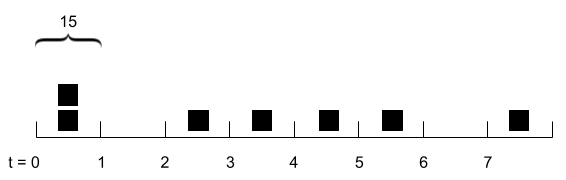
\includegraphics{schedule.png}

}

\caption{A schedule
\(X = [2, 0, 1, 1, 1, 1, 0, 1], T = 8, N = 7, d = 15\)}

\end{figure}

Each patient has two endogenous features: type and service time, which
are both indepent and identically distributed variables. In our model we
assume there are two patient types: standard and emergency. There is a
probability \(q\) that a patient has an emergency. Service times have
known distributions with mean \(\beta_s\) and \(\beta_e\) for standard
and emergency patients respectively.

All standard patients are assumed to be punctual. The arrival rate of
emergency patients has a Poisson distribution with mean \(\lambda\).
Emergency patients get priority over standard patients that are waiting.
If several emergency patients are waiting they are served in order of
arrival.

The cost function consists of three elements:

\begin{enumerate}
\def\labelenumi{\arabic{enumi}.}
\tightlist
\item
  The waiting time for patients: \(W(x)\)
\item
  The waiting or idle time for physicians: \(I(x)\)
\item
  The lateness or over-time of physicians: \(L(x)\)
\end{enumerate}

and becomes:

\[
C(x) = \alpha W(x) + \beta I(x) + \gamma L(x)
\]

The weights \(\alpha, \beta,\gamma \geq0\) can be set to reflect the
relative importance of each cost element.

The problem is to find a schedule \(X\) that minimizes the cost function
\(C(x)\):

\[
min\{C(x)|\displaystyle\sum_{t=0} ^{T-1} x_t = N, x_t \in \mathbb{N}_0\}
\]

\hypertarget{results}{%
\section{Results}\label{results}}

Results and Discussion can be combined.

Nulla mi mi, venenatis sed ipsum varius, Table~\ref{table1} volutpat
euismod diam. Proin rutrum vel massa non gravida. Quisque tempor sem et
dignissim rutrum. Lorem ipsum dolor sit amet, consectetur adipiscing
elit. Morbi at justo vitae nulla elementum commodo eu id massa. In vitae
diam ac augue semper tincidunt eu ut eros. Fusce fringilla erat
porttitor lectus cursus, \nameref{s1-video} vel sagittis arcu lobortis.
Aliquam in enim semper, aliquam massa id, cursus neque. Praesent
faucibus semper libero.

% Place tables after the first paragraph in which they are cited.
\begin{table}[!ht]
\begin{adjustwidth}{-2.25in}{0in} % Comment out/remove adjustwidth environment if table fits in text column.
\centering
\caption{
{\bf Table caption Nulla mi mi, venenatis sed ipsum varius, volutpat euismod diam.}}
\begin{tabular}{|l+l|l|l|l|l|l|l|}
\hline
\multicolumn{4}{|l|}{\bf Heading1} & \multicolumn{4}{|l|}{\bf Heading2}\\ \thickhline
$cell1 row1$ & cell2 row 1 & cell3 row 1 & cell4 row 1 & cell5 row 1 & cell6 row 1 & cell7 row 1 & cell8 row 1\\ \hline
$cell1 row2$ & cell2 row 2 & cell3 row 2 & cell4 row 2 & cell5 row 2 & cell6 row 2 & cell7 row 2 & cell8 row 2\\ \hline
$cell1 row3$ & cell2 row 3 & cell3 row 3 & cell4 row 3 & cell5 row 3 & cell6 row 3 & cell7 row 3 & cell8 row 3\\ \hline
\end{tabular}
\begin{flushleft} Table notes Phasellus venenatis, tortor nec vestibulum mattis, massa tortor interdum felis, nec pellentesque metus tortor nec nisl. Ut ornare mauris tellus, vel dapibus arcu suscipit sed.
\end{flushleft}
\label{table1}
\end{adjustwidth}
\end{table}

\hypertarget{lorem-and-ipsum-nunc-blandit-a-tortor}{%
\subsection{\texorpdfstring{\textbf{LOREM}~and \textbf{IPSUM}~nunc
blandit a
tortor}{LOREM~and IPSUM~nunc blandit a tortor}}\label{lorem-and-ipsum-nunc-blandit-a-tortor}}

\hypertarget{rd-level-heading}{%
\subsubsection{3rd level heading}\label{rd-level-heading}}

Maecenas convallis mauris sit amet sem ultrices gravida. Etiam eget
sapien nibh. Sed ac ipsum eget enim egestas ullamcorper nec euismod
ligula. Curabitur fringilla pulvinar lectus consectetur pellentesque.
Quisque augue sem, tincidunt sit amet feugiat eget, ullamcorper sed
velit. Sed non aliquet felis. Lorem ipsum dolor sit amet, consectetur
adipiscing elit. Mauris commodo justo ac dui pretium imperdiet. Sed
suscipit iaculis mi at feugiat.

\begin{enumerate}
\def\labelenumi{\arabic{enumi}.}
\item
  react
\item
  diffuse free particles
\item
  increment time by dt and go to 1
\end{enumerate}

\hypertarget{sed-ac-quam-id-nisi-malesuada-congue}{%
\subsection{Sed ac quam id nisi malesuada
congue}\label{sed-ac-quam-id-nisi-malesuada-congue}}

Nulla mi mi, venenatis sed ipsum varius, volutpat euismod diam. Proin
rutrum vel massa non gravida. Quisque tempor sem et dignissim rutrum.
Lorem ipsum dolor sit amet, consectetur adipiscing elit. Morbi at justo
vitae nulla elementum commodo eu id massa. In vitae diam ac augue semper
tincidunt eu ut eros. Fusce fringilla erat porttitor lectus cursus, vel
sagittis arcu lobortis. Aliquam in enim semper, aliquam massa id, cursus
neque. Praesent faucibus semper libero.

\begin{itemize}
\item
  First bulleted item.
\item
  Second bulleted item.
\item
  Third bulleted item.
\end{itemize}

\hypertarget{discussion}{%
\section{Discussion}\label{discussion}}

Nulla mi mi, venenatis sed ipsum varius,see Table~\ref{table1} volutpat
euismod diam. Proin rutrum vel massa non gravida. Quisque tempor sem et
dignissim rutrum. Lorem ipsum dolor sit amet, consectetur adipiscing
elit. Morbi at justo vitae nulla elementum commodo eu id massa. In vitae
diam ac augue semper tincidunt eu ut eros. Fusce fringilla erat
porttitor lectus cursus, vel sagittis arcu lobortis. Aliquam in enim
semper, aliquam massa id, cursus neque. Praesent faucibus semper libero.

\hypertarget{conclusion}{%
\section{Conclusion}\label{conclusion}}

CO\textsubscript{2} Maecenas convallis mauris sit amet sem ultrices
gravida. Etiam eget sapien nibh. Sed ac ipsum eget enim egestas
ullamcorper nec euismod ligula. Curabitur fringilla pulvinar lectus
consectetur pellentesque. Quisque augue sem, tincidunt sit amet feugiat
eget, ullamcorper sed velit.

Sed non aliquet felis. Lorem ipsum dolor sit amet, consectetur
adipiscing elit. Mauris commodo justo ac dui pretium imperdiet. Sed
suscipit iaculis mi at feugiat. Ut neque ipsum, luctus id lacus ut,
laoreet scelerisque urna. Phasellus venenatis, tortor nec vestibulum
mattis, massa tortor interdum felis, nec pellentesque metus tortor nec
nisl. Ut ornare mauris tellus, vel dapibus arcu suscipit sed. Nam
condimentum sem eget mollis euismod. Nullam dui urna, gravida venenatis
dui et, tincidunt sodales ex. Nunc est dui, sodales sed mauris nec,
auctor sagittis leo. Aliquam tincidunt, ex in facilisis elementum,
libero lectus luctus est, non vulputate nisl augue at dolor. For more
information, see \nameref{s1-appendix}.

\hypertarget{supporting-information}{%
\section{Supporting information}\label{supporting-information}}

\paragraph*{S1 Fig.}
\label{s1-fig}
{\textbf{Bold the title sentence.}} Add descriptive text after the title
of the item (optional).

\paragraph*{S2 Fig.}
\label{s2-fig}
{\textbf{Lorem ipsum.}} Maecenas convallis mauris sit amet sem ultrices
gravida. Etiam eget sapien nibh. Sed ac ipsum eget enim egestas
ullamcorper nec euismod ligula. Curabitur fringilla pulvinar lectus
consectetur pellentesque.

\paragraph*{S1 File.}
\label{s1-file}
{\textbf{Lorem ipsum.}}

\paragraph*{S1 Video.}
\label{s1-video}
{\textbf{Lorem ipsum.}} Maecenas convallis mauris sit amet sem ultrices
gravida. Etiam eget sapien nibh. Sed ac ipsum eget enim egestas
ullamcorper nec euismod ligula. Curabitur fringilla pulvinar lectus
consectetur pellentesque.

\paragraph*{S1 Appendix.}
\label{s1-appendix}
{\textbf{Lorem ipsum.}} Maecenas convallis mauris sit amet sem ultrices
gravida. Etiam eget sapien nibh. Sed ac ipsum eget enim egestas
ullamcorper nec euismod ligula. Curabitur fringilla pulvinar lectus
consectetur pellentesque.

\paragraph*{S1 Table.}
\label{s1-table}
{\textbf{Lorem ipsum.}} Maecenas convallis mauris sit amet sem ultrices
gravida. Etiam eget sapien nibh. Sed ac ipsum eget enim egestas
ullamcorper nec euismod ligula. Curabitur fringilla pulvinar lectus
consectetur pellentesque.

\hypertarget{acknowledgments}{%
\section{Acknowledgments}\label{acknowledgments}}

Cras egestas velit mauris, eu mollis turpis pellentesque sit amet.
Interdum et malesuada fames ac ante ipsum primis in faucibus. Nam id
pretium nisi. Sed ac quam id nisi malesuada congue. Sed interdum aliquet
augue, at pellentesque quam rhoncus vitae.


\nolinenumbers
  \bibliography{bibliography.bib}

\end{document}
